% \begin{spverbatim}
%1LiDAR配置の図
\deleted{Fig.~\ref{jlidar} shows the deployment of the devices for the experiment.}
%2具体的な配置方法
%blue
The two LiDAR sensors were placed on a table facing each other.
\deleted{They were positioned 1.0 m away from the subject in a lateral direction and tilted down by $10^{\circ}$ to make the PC easier to detect.}
\revised{They were positioned 1.0 m away from the experiment participant in a lateral direction and tilted down by $10^{\circ}$ to make the PC easier to detect.}
\deleted{The PC was placed on the table in front of the subject.}
\revised{The PC was placed on the table in front of the experiment participant.} 
%3実験の様子
Fig.~\ref{experimentsite} shows the experiment site. 
  
% \end{spverbatim}

\begin{figure}[t]
  \centering
  {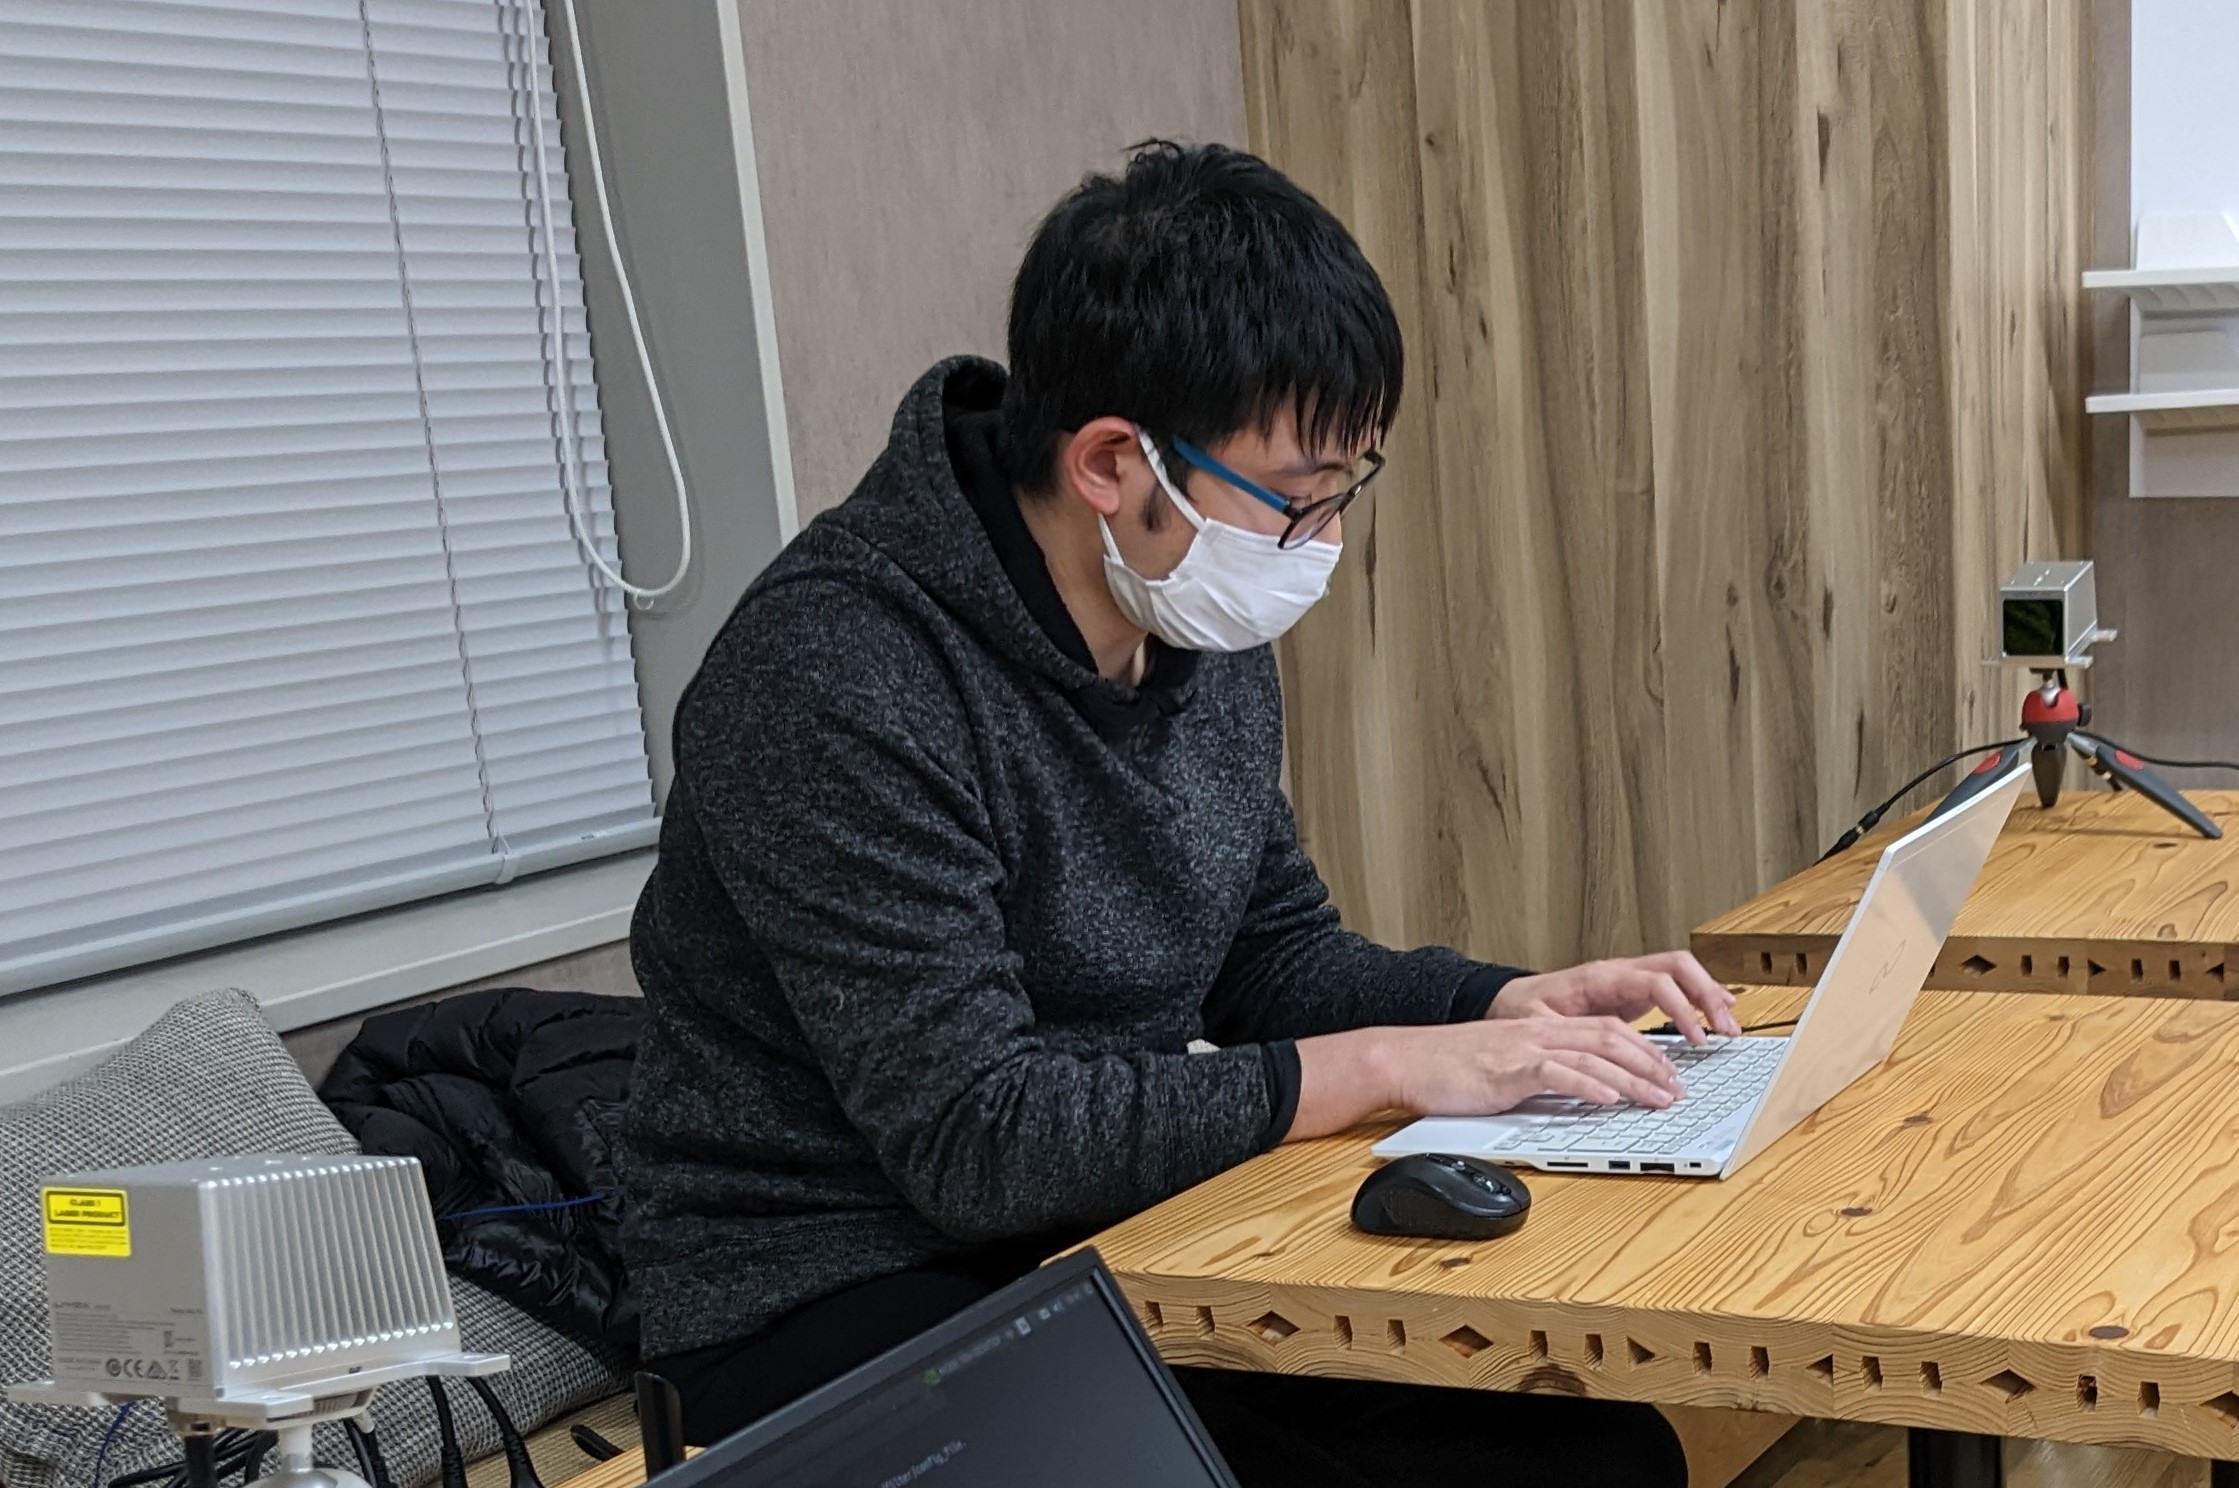
\includegraphics[width=\linewidth]{img/experimentsite2.jpg}}
  \caption{Experiment site.}
  \label{experimentsite}
\end{figure}

\begin{deletedblock}
\begin{figure}[t]
  \centering
  {
\includegraphics[width=\linewidth]{img/ld_journal5.drawio.png}}
  \caption{Deployment of LiDAR sensors.}
  \label{jlidar}
\end{figure}
\end{deletedblock}